
%%%%%%%%%%%%%%%%%%%%%%%%%%%%%%%%%%%%%%%%%%%%%%%%%%%%
%%%             Metadata                         %%%
%%%%%%%%%%%%%%%%%%%%%%%%%%%%%%%%%%%%%%%%%%%%%%%%%%%%      

\title{Grundkurs Linguistik}

\subtitle{Semantik}

%\toggletrue{uebung}

\exewidth{\exnrfont(235)}


\author{Stefan Müller}


\section{Semantik}

\huberlintitlepage

\frame{
\frametitle{Semantik: Material}


\citew{Zimmermann2001a-u}


}

\author{Stefan Müller (Ede Zimmermann)}

\outline{

\begin{itemize}
\item Ebenen linguistischer Analyse
\item Wörtliche Bedeutung: Abgrenzunug zur Pragmatik
\item Lexikalische Semantik
\item Satzsemantik
\end{itemize}

}


\subsection{Abgrenzung}

\begin{frame}{Rekapitulation: Ebenen linguistischer Analyse}

  \begin{itemize}
  \item Phonetik/Phonologie\\
Welche Eigenschaften haben Laute und Töne einer Sprache, welchen Regeln unterliegen sie, und welche dieser Eigenschaften dienen in einer Sprache dazu, Bedeutungen zu unterscheiden?

  \item<2-> Morphologie\\
   Welche Lautkombinationen haben eine Bedeutung und\\ nach welchen Regeln lassen sich diese zu Wörtern zusammensetzen?

  \item<3-> Syntax\\
 Nach welchen Regeln lassen sich Wörter zu Satzteilen und Satzteile zu ganzen Sätzen zusammenfügen?

  \item<4-> Semantik\\
 Welche Bedeutung haben Wörter bzw.\ Morpheme und nach welchen Regeln lässt sich die Bedeutung von Wörtern,
 Satzteilen und Sätzen aus der Bedeutung der Einzelteile (Morpheme, Wörter, andere Satzteile) erschließen?
  \end{itemize}
\end{frame}


\subsection{Wörtliche Bedeutung}

\outline{

\begin{itemize}
\item Ebenen linguistischer Analyse
\item \blaubf{Wörtliche Bedeutung: Abgrenzunug zur Pragmatik}
\item Lexikalische Semantik
\item Satzsemantik
\end{itemize}

}


\frame{
\frametitlefit{Wörtliche Bedeutung -- Verborgener Sinn, Ironie, Implikatur}


\begin{itemize}
\item Den Untersuchungsgegenstand der Semantik bilden sprachliche Inhalte bzw.\ \blaubf{Sinn} und
  \blaubf{Bedeutung} (Wir unterscheiden terminologisch nicht zwischen Sinn und Bedeutung).
\pause
\item Nicht alles, was man mit einer Äußerung assoziiert, gehört zur Semantik.
\begin{itemize}
\item Verborgener Sinn (Gedichte)
\pause
\item Ironie und Implikatur
\eal
\ex Das Steak war wie immer zart und saftig.\\(je nach Mensa ironisch)
\ex Der Nachtisch war nicht giftig.\\(Implikatur je nach Kontext $\to$ schlecht)
\zl
\end{itemize}
\end{itemize}

}

\frame{
\frametitle{Wörtliche Bedeutung -- Stil, Metaphern}

\begin{itemize}
\item Nicht alles, was man mit einer Äußerung assoziiert, gehört zur Semantik.
\begin{itemize}
\item Wortwahl und Stil kann Sprechereinstellungen übermitteln:
\eal
\ex Willst Du allen Ernstes für den Fraß noch mehr Kohle verlangen?
\ex Planen Sie tatsächlich eine Anhebung der Essenspreise?
\zl
(duzen, \emph{Fraß}, \emph{wollen} unhöflich, \emph{allen Ernstes} abwegig?, \emph{Kohle} Slang)

\pause
\item Sprachliche Bilder (Metaphern):
\eal
\ex Fußballer = Terrier (Laufstil, Aussehen, Charakter)
\ex Klagelied meines Kühlschranks
\zl

Geräusch des Kühlschranks klingt wie Klagelied $\to$ Vergleich\\
(\mex{0}b) ist dagegen eine Metapher, da offen bleibt,\\
worin der Vergleich besteht (Geräusch, Kühlschrank leer, \ldots).

\end{itemize}
\end{itemize}

}

\frame{
\frametitle{Metaphern}

\begin{itemize}
\item Metaphern können verblassen und eine wörtliche Bedeutung annehmen:
\ea
fadenscheinig
\z
Zusätzlich zur alten Bedeutung (Qualität eines Gewebes) gibt es eine neue: Qualität der
Selbstrechtfertigung.

\pause
Man sagt, die Metapher ist \blaubf{erstarrt}.

\pause
\item Was ist der wörtliche Sinn von (\mex{1})?
\ea
Die Ausflüchte des Terriers waren fadenscheinig.
\z
Nur \emph{Terrier} ist metaphorisch verwendet, \emph{fadenscheinig} ist in wörtlicher Lesart
verwendet worden:
\ea
Ein Hund hat schlechte Ausreden vorgebracht.
\z


\end{itemize}

}

\begin{frame}
\frametitle{Metapher oder nicht?}
  \begin{itemize}
  \item Wann ist eine Metapher erstarrt?\\
        Das kann man nicht genau festlegen, da die Übergänge fließend sind.
\pause
\item Trotzdem ist eine scharfe Trennung für bestimmte Zwecke sinnvoll:\\ semantische Theoriebildung.
\pause
\item Abgrenzung erlaubt getrennte Bearbeitung der Bereiche,\\ mit verschiedenen Methoden.
\pause
\item Semantik beschäftigt sich mit der wörtlichen Bedeutung und alles was über den reinen Wortsinn
  hinausgeht ist Gegenstand der Pragmatik.
  \end{itemize}
\end{frame}

\subsection{Lexikalische Semantik}

\outline{

\begin{itemize}
\item Ebenen linguistischer Analyse
\item Wörtliche Bedeutung: Abgrenzunug zur Pragmatik
\item \blaubf{Lexikalische Semantik}
\item Satzsemantik
\end{itemize}

}


\begin{frame}
\frametitle{Lexikalische Semantik}

  \begin{itemize}
  \item Die Bedeutung eines komplexen Ausdrucks ergibt sich aus der Bedeutung seiner Teile + der
    Art, wie diese kombiniert wurden.

\pause

\item Das nennt man \blaubf{Frege-Prinzip}.
%, obwohl Frege es selbst in seinen Texten nicht explizit formuliert hat.

% Antonio:
%% It is astonishing what language accomplishes. With a few syllables it expresses a countless
%% munber of thoughts, and even for a thought grasped for the first time by a human it provieles a
%% clothing in which it can be recognized by another to whom it is entirely new. This would not be
%% possible if we could not distinguish parts in the thought that correspond to parts of the
%% sentence, so that the construction of the sentence can be taken to mirror the construction of the
%% thought. ... If we thus view thoughts as composed of simple parts and take these, in turn, to
%% correspond to simple sentence-parts, we can understand how a few sentence-parts can go to make up
%% a great multitude of sentences to which, in turn, there correspond a great multitude of
%% thoughts. The question now arises how the construction of the thought proceeds, and by what means
%% the parts are put tagether so that the whole is something more than the isolated parts. In my
%% essay "Negation," I considered the. case of a thought that appears to be composed of one part
%% which is in need of completion or, as one might say, unsaturated, and whose linguistic correlate
%% is the negative particle, and another part which is a thought. We cannot negate without negating
%% something, and this something is a thought. Because this thought saturates the unsaturated part
%% or, as one might say, completes what is in need of completion, the whole hangs together. And it
%% is a natural conjecture that logical combination of parts into a whole is always a matter of
%% saturating something unsaturated.  G. Frege, "Logische Untersuchungen. Dritter Teil:
%% Geclankengefüge," Beiträge zur Philosophie des deutschen Idealismus, 3 (1923-6), pp. 36-51.

\pause
  \item Frage: Was bedeuten die Teile?

    \bigskip
    
    \pause
    	\item Wortbedeutung \ras konventionalisierter und kontextunabhängiger Inhalt eines Ausdrucks
\pause
	\item Lexikalische Semantik:
	
	\begin{itemize}
		\item Erfassung des invariablen Inhalts eines Wortes
		\item Repräsentation und Organisation des Inhalts
	\end{itemize}
	
\pause
	\item Siehe: Merkmalshypothese, Prototypentheorie, Wortfeldrelationen, etc.


  \end{itemize}
\end{frame}


%\author{Antonio MyP}


\subsubsection{Homonymie}

\begin{frame}
\frametitle{Homonymie und grammatische Eigenschaften}

\begin{itemize}
  \item Es ist möglich, dass ein "`Wort"' mehrere Lesarten hat.

Man spricht dann von \blaubf{Homonymie}: 
\eal
\ex der/die Kiefer -- die Kiefer/die Kiefern
\pause
\ex der/das Bauer -- die Bauern/die Bauer
\pause
\ex \visible<4->{das} {Band} \pause\visible<4->{({Bänder}) -- der {Band} ({Bände}) -- die {Band} ({Bands})}
\zl

Die Wörter unterscheiden sich im Genus.

  \end{itemize}
\end{frame}




\frame{
\frametitle{Homonymie: Plural}

\begin{columns}[T]

\begin{column}{45mm}
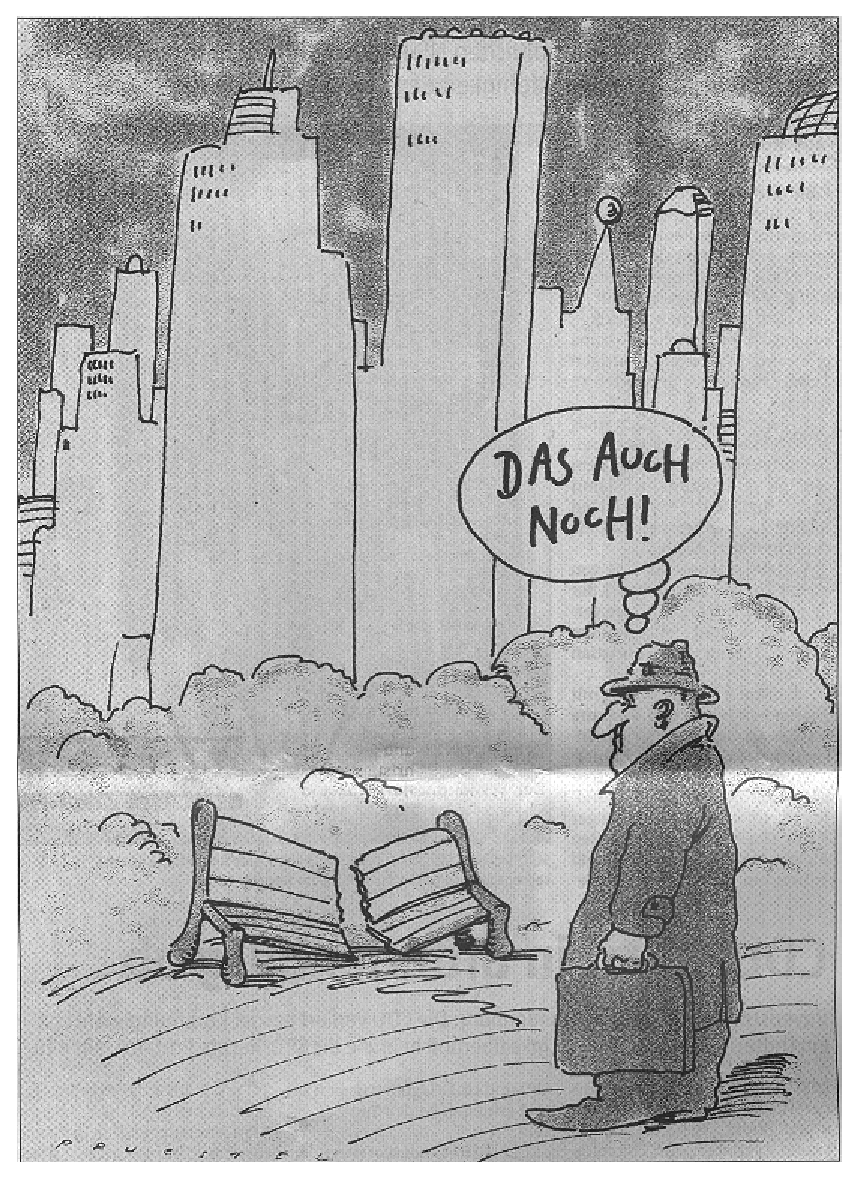
\includegraphics[width=\textwidth]{Bilder/bankenkrise}
\end{column}
\begin{column}{73mm}
Genusunterschiede nicht immer gegeben:
\eal
\ex die Bank -- die Banken
\ex die Bank -- die Bänke
\zl
\end{column}
\end{columns}
}

\frame{
\frametitle{Homonymie: grammatisch unmarkiert}


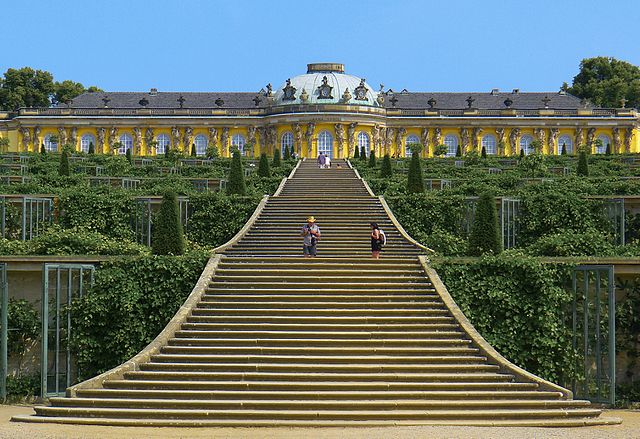
\includegraphics[width=0.6\textwidth]{material/Potsdam_sans_souci}\hfill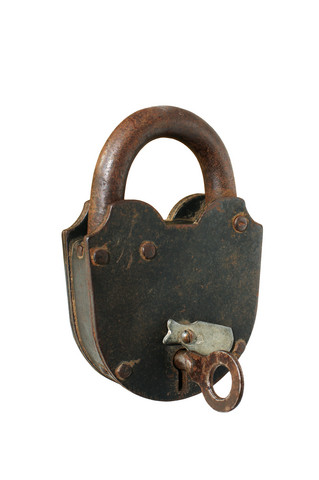
\includegraphics[width=0.3\textwidth]{material/Schloss_alt}

Wieviele Schlösser sind hier zu sehen? \\
{\scriptsize (\url{https://commons.wikimedia.org}; www.colourbox.de)}

}

%\subsubsection{Homophone und Homographen}

\begin{frame}
\frametitle{Homophone und Homographen}
  \begin{itemize}
  \item \blaubf{Homophone}
\eal
\ex Miene (Gesichtsausdruck) 
\ex Mine (Bergwerk, Sprengkörper, Stift) 
\zl
\pause
\item \blaubf{Homographen} 
\eal 
\ex übers\textprimstress etzen 
\ex \textprimstress übersetzen
\zl
\pause
\item Solche Identität von Formen ist aber relativ uninteressant,\\
      weil zufällig oder historisch begründet.
  \end{itemize}
\end{frame}


\subsubsection{Polysemie}

\begin{frame}
\frametitle{Polyseme}
  \begin{itemize}
  \item Interessanter sind Polyseme:
\eal
\ex Krone: Königskrone, Baumkrone, Schaumkrone
\ex belegen: ein Seminar/einen Platz/eine Aussage/ein Brötchen belegen
\zl
Die Lesarten unterscheiden sich, sind aber miteinander verwandt.

\pause
\item Produktive Polysemien interessant, weil sich dafür Regeln finden lassen.

% Wikipedia Metonymie
%
Beispiel: \blaubf{Metonymie} (Namensvertauschung, Umbennenung): gemeinter Gegenstand wird durch einen Ausdruck bezeichnet, der sich
auf einen anderen, aber verbundenen Gegenstand bezieht. \zb Teil für Ganzes.
\ea
Möchtest Du noch eine Tasse? = \\Möchtest Du noch eine Tasse gefüllt mit Tee?
\z
Genauso \emph{Glas}, \emph{Teller}: Gefäß für Inhalt

% Meronymie = Finger Hand
% (auch Meronymie, méros = Teil)
  \end{itemize}
\end{frame}

\begin{frame}
\frametitle{Polysemie}
  \begin{itemize}
  \item Tier für sein Fleisch.
\eal
\ex Dort drüben läuft ein Kaninchen. 
\ex Zu Ostern gab es Kaninchen.
\zl
  \end{itemize}
\end{frame}




%%%%%%%%%%%%%%%%%%%%%%%%%%%%%%%%%%%
%
\subsubsection{Sinnrelationen}
%
%\frame{
%\begin{multicols}{2}
%\frametitle{~}
%	\tableofcontents[currentsection]
%\end{multicols}
%}
%%%%%%%%%%%%%%%%%%%%%%%%%%%%%%%%%%%%%%%

\begin{frame}
\frametitle{Sinnrelationen}

\begin{itemize}
	\item Zusammenhang zwischen den Bedeutungen von Ausdrücken
	\item Systematisch erfassbare Relationen:
	
\vspace{5mm}
	
	\begin{itemize}
		\item Synonymie
		\item Hyponymie / Hyperonymie (Kohyponymie)
		\item Meronymie
 		\item Antonymie
	\end{itemize}
	
\end{itemize}

\end{frame}


%%%%%%%%%%%%%%%%%%%%%%%%%%%%%%%%%%%

\begin{frame}
\frametitle{Synonymie}

\begin{itemize}
	\item Zwei Ausdrücke X und Y sind Synonyme, wenn der Austausch von X durch Y und umgekehrt in allen Kontexten bei Wahrung der Wahrheit (salva veritate) erfolgt.
	\item[]
	\item Bikonditional: $\leftrightarrow$
	
	\eal
		\ex Apfelsine $\leftrightarrow$ Orange
		\ex anfangen $\leftrightarrow$ beginnen
		\ex sterben $\leftrightarrow$ abkratzen (in einer Bedeutung)
		\ex Treppe $\leftrightarrow$ Stiege
		\ex Brötchen $\leftrightarrow$ Schrippe $\leftrightarrow$ Semmel
	\zl
	
	\item Konnotative, regionale und registerabhängige Unterschiede
\end{itemize}

\end{frame}


%%%%%%%%%%%%%%%%%%%%%%%%%%%%%%%%%%%

\begin{frame}
\frametitle{Hyperonymie / Hyponymie}

\begin{itemize}
	\item 
Ein Ausdruck X ist ein Hyperonym von Y,\\
wenn die Bedeutung von Y in der Bedeutung von X enthalten ist.

Ein Ausdruck Y ist ein Hyponym von X,\\
wenn die Bedeutung von Y in der Bedeutung von X enthalten ist.
	\item[]	
	\item Transitive Relation
	\item[]
	\item Implikation: \ras
	
	\begin{itemize}
		\item Y ist ein X
		
		\eal 
		\ex Küchenstuhl \ras Stuhl \ras Sitzgelegenheit
		\ex erschie\ss{}en \ras töten
		\zl
		
	\end{itemize}
	
\end{itemize}

\end{frame}


%%%%%%%%%%%%%%%%%%%%%%%%%%%%%%%%%%%

\begin{frame}
\frametitle{Kohyponymie}

\begin{itemize}
\item
  Ein Ausdruck X ist ein Kohyponym von Z (und umgekehrt),\\
wenn die Bedeutung von X und Z in der Bedeutung von Y enthalten ist. 

Kohyponyme schließen einander aus (Inkompatibilität)

\eal
\ex Drehstuhl $|$ Küchenstuhl \ras Stuhl \ras Sitzgelegenheit
\ex erschießen / erwürgen / erdrosseln \ras töten
\zl


	\item[]
	\item Hyperonymie $|$ Hyponymie: Basis für Taxonomien

\end{itemize}

\end{frame}


%%%%%%%%%%%%%%%%%%%%%%%%%%%%%%%%%%

\begin{frame}
\frametitle{Meronymie}

\begin{itemize}
	\item 
Ein Ausdruck X ist ein Meronym von Y, wenn X ein Teil von Y ist.

\vspace{5mm}
	
	\eal
	\ex Finger > Hand > Arm > Oberkörper > Körper
	\ex Rad > Auto
	\zl

	\item scheint transitiv zu sein: 
		
	\ea die Manschette des Ärmels, der Ärmel der Jacke \ras die Manschette der Jacke
	\z
		
	\item Ist aber intransitiv: 
		
	\ea der Griff der Tür, die Tür des Hauses \ras \# der Griff des Hauses
	\z
		
\end{itemize}

\end{frame}


%%%%%%%%%%%%%%%%%%%%%%%%%%%%%%%%%%%

\begin{frame}
\frametitle{Antonymie}

\begin{itemize}
	\item 
Ein Ausdruck X ist ein Antonym von Y,\\
wenn X in irgendeinem Sinne das Gegenteil von Y ist.
	\item[]	
	\item X \ras $\lnot$ Y
	
	\eal 
		\ex fleißig -- faul
		\ex klug -- dumm
	\zl
	
\end{itemize}

\end{frame}


%%%%%%%%%%%%%%%%%%%%%%%%%%%%%%%%%%%

\begin{frame}
\frametitle{Kontradiktorische Antonymie}

\begin{itemize}
	\item 
Ein Ausdruck X ist ein kontradiktorisches Antonym von Y,\\
wenn die Negation von X die Bedeutung von Y ergibt und umgekehrt.\\
(Eine drittes Z ist ausgeschlossen)
	\item Komplementarität: (X \ras $\lnot$ Y) \& ($\lnot$ X  \ras Y)
	\item Binär
	\item Beide Aussagen können nicht gleichzeitig wahr sein und auch nicht gleichzeitig falsch sein.
	
	\eal
		\ex krank -- gesund
		\ex lebendig -- tot
		\ex anwesend -- abwesend
	\zl
	
\end{itemize}

\end{frame}


%%%%%%%%%%%%%%%%%%%%%%%%%%%%%%%%%%%

\begin{frame}
\frametitle{Konträre Antonymie}

\begin{itemize}
	\item
Ein Ausdruck X ist ein konträres Antonym von Y,\\
wenn X und Y nicht zugleich wahr sein können,\\
aber beide können zugleich nicht zutreffen.
	\item[]
	\item Skalar: Antonymie mit Zwischenstufen
	\item[]
	\item Beide Aussagen können nicht gleichzeitig wahr sein,\\
              aber sie können gleichzeitig falsch sein.
	\item[]
	\item (X $\rightarrow \lnot$ Y) \& (Y $\rightarrow \lnot$ X)
	
	\eal
		\ex reich -- arm
		\ex kalt -- (kühl -- lau -- warm) -- heiß
	\zl
	
\end{itemize}

\end{frame}


%% %%%%%%%%%%%%%%%%%%%%%%%%%%%%%%%%%%%

%% \begin{frame}
%% \frametitle{Sinnrelationen}

%% \begin{itemize}
%% 	\item \textbf{Ambiguität (Lexikalische Mehrdeutigkeit)}

%% \vspace{1em}

%% 	\begin{itemize}
%% 		\item \textbf{Homonymie}\\
%% Ein Ausdruck X und ein Ausdruck Y sind gleich in deren Form (phonetische oder graphische) aber unterschiedlich in deren Bedeutung, wobei X und Y unterschiedliche Ursprünge haben.
%% 	\end{itemize}
%% \end{itemize}

%% \end{frame}


%% %%%%%%%%%%%%%%%%%%%%%%%%%%%%%%%%%%%

%% \begin{frame}
%% \frametitle{Sinnrelationen}

%% \begin{itemize}
%% 	\item \textbf{Ambiguität (Lexikalische Mehrdeutigkeit)}

%% \vspace{1em}

%% 	\begin{itemize}
%% 		\item \textbf{Homonymie:}
		
%% 		\begin{itemize}
%% 			\item Homophonie:
			
%% 			\eal
%% 			\ex mahlen vs. malen 
%% 			\ex sieben (7) vs. sieben
%% 			\ex laut vs. laut (Präp.)
%% 			\zl
			
%% 			\item Homographie:
					
%% 			\eal 
%% 			\ex 'modern vs. mo'dern
%% 			\ex Die Therapie des gebrochenen Beines beinhaltet das Fixieren in einer Beinhalterung.
%% 			\zl
			
%% 		\end{itemize}
		
%% 	\end{itemize}
%% \end{itemize}

%% \end{frame}


%% %%%%%%%%%%%%%%%%%%%%%%%%%%%%%%%%%%%

%% \begin{frame}
%% \frametitle{Sinnrelationen}

%% \begin{itemize}
%% 	\item \textbf{Ambiguität (Lexikalische Mehrdeutigkeit)}
	
%% \vspace{1em}

%% 	\begin{itemize}
%% 		\item \textbf{Polysemie}\\
%% Ein Ausdruck X und ein Ausdruck Y sind gleich in deren Form (phonetische und graphische) können aber unterschiedliche Bedeutungsvarianten voneinander sein. X und Y stehen in einem etymologischen Zusammenhang zueinander.

%% 		\ea Schule, Oper, Grammatik
%% 		\z

%% 	\end{itemize}
	
%% \end{itemize}

%% \end{frame}


%%%%%%%%%%%%%%%%%%%%%%%%%%%%%%%%%%%
\iftoggle{uebung}{

\begin{frame}
\frametitle{Sinnrelationen}

\begin{itemize}
	\item \textbf{Übung:}
	
	\eal
	\ex Ballkleid -- Kleid
	\ex Bank -- Bank
	\ex Schraubenzieher -- Zange
	\ex gro\ss{} -- klein
	\ex Henkel -- Tasse
	\ex Ahorn -- Baum
	\ex essen -- verzehren
	\ex gerade -- ungerade
	\zl
		
\end{itemize}

\end{frame}


%%%%%%%%%%%%%%%%%%%%%%%%%%%%%%%%%%%%%%%%%
%\iftoggle{loesung}{

\begin{frame}
\frametitle{Sinnrelationen: Lösung}
	
	\eal
	\ex Ballkleid -- Kleid: Hyponym/Hyperonym
	\ex Bank -- Bank: Homonymie (-graphie und -phonie)
	\ex Schraubenzieher -- Zange: Kohyponymie
	\ex gro\ss{} -- klein: Konträre Antonymie
	\ex Henkel -- Tasse: Meronymie
	\ex Ahorn -- Baum: Hyponym/Hyperonym
	\ex essen -- verzehren: Synonymie
	\ex gerade -- ungerade: Kontradiktorische Antonymie
	\zl

\end{frame}
%}

}

%%%%%%%%%%%%%%%%%%%%%%%%%%%%%%%%%%%%%%%%%%%
%
\subsection{Satzsemantik (Satzbedeutung)}
%
\iftoggle{toc}{
\frame{
\begin{multicols}{2}
\frametitle{~}
	\tableofcontents[currentsection]
\end{multicols}
}
}
%%%%%%%%%%%%%%%%%%%%%%%%%%%%%%%%%%%%%%%%%%

\outline{

\begin{itemize}
\item Ebenen linguistischer Analyse
\item Wörtliche Bedeutung: Abgrenzunug zur Pragmatik
\item Lexikalische Semantik
\item \blaubf{Satzsemantik}
\end{itemize}

}



\begin{frame}
\frametitle{Satzsemantik (Satzbedeutung)}

\begin{itemize}
	\item Wahrheitsbedingungen (\citeauthor{Wittgenstein72a-u} 1921)
	\item[]
	\item Die Bedeutung eines Satzes zu kennen, heißt, notwendige und hinreichende Bedingungen für die Wahrheit bzw. Falschheit des Satzes (= seine Wahrheitsbedingungen) zu kennen.
	\item[]
	\item Bedingungen in der aktuellen Welt (verschiedene Welten)
	
	
		\ea Martin kauft Brötchen.
		\z
		
	\begin{itemize}	
		\item Wahr oder Falsch (1 oder 0) \ras abhängig von der Welt
	\end{itemize}
	
\end{itemize}

\end{frame}


%%%%%%%%%%%%%%%%%%%%%%%%%%%%%%%%%%%%%%%%%%

\begin{frame}
\frametitle{Satzsemantik (Satzbedeutung)}

\begin{itemize}
	\item \textbf{Kompositionalitätsprinzip}\\
Die Bedeutung eines komplexen Ausdrucks ergibt sich aus der Bedeutung seiner unmittelbaren syntaktischen Teile und der Art und Weise, wie sie sich syntaktisch zusammensetzen.
	\item[]
	\item Auch Fregeprinzip genannt
\end{itemize}

\end{frame}


%%%%%%%%%%%%%%%%%%%%%%%%%%%%%%%%%%%%%%%%%%
%%%%%%%%%%%%%%%%%%%%%%%%%%%%%%%%%%%%%%%%%%
%
\subsubsection{Aussagenlogik}
%\frame{
%\begin{multicols}{2}
%\frametitle{~}
%	\tableofcontents[currentsection]
%\end{multicols}
%}
%%%%%%%%%%%%%%%%%%%%%%%%%%%%%%%%%%%%%%%%%%


\begin{frame}
\frametitle{Aussagenlogik}

\begin{itemize}
	\item Basierend auf dem Kompositionalitätsprinzip
	\item Teilgebiet der formalen Logik
	\item Verknüpfung von einfachen Aussagen
	\item Wie lässt sich der Wahrheitswert einer komplexen Aussage aus den Wahrheitswerten der in ihr enthaltenen einfachen Aussagen in Abhängigkeit der Verknüpfung errechnen?
\end{itemize}

\end{frame}


%%%%%%%%%%%%%%%%%%%%%%%%%%%%%%%%%%%%%%%%%%

\subsubsubsection{Konnektoren}

\begin{frame}
\frametitle{Konnektoren}

\begin{itemize}
	\item Aussagen: p, q, r, s, \dots
	\item Konnektoren:
	
	\begin{itemize}
		\item Negation (NICHT): $\lnot$
		
		\item Konjunktion (UND): $\land$
		
		\item Disjunktion (UND/ODER): $\lor$
		
		\item Konditional (materiale Implikation) (WENN, DANN): \ras
		
		\item Bikonditional (GENAU DANN WENN): $\leftrightarrow$
	\end{itemize}
	
\end{itemize}

\end{frame}


%%%%%%%%%%%%%%%%%%%%%%%%%%%%%%%%%%%%%%%%%%

\begin{frame}
\frametitle{Negation}

\begin{itemize}
	\item Negation (NICHT): $\lnot$
	
	\eal
		\ex p: Es regnet.
		\ex $\lnot$ p: Es regnet nicht.
	\zl
	
\end{itemize}

\begin{table}
\centering
\begin{tabular}{p{3cm}|p{3cm}}
\textbf{p} & \textbf{$\lnot$p}\\
\hline
1 & 0\\
\hline
0 & 1\\
\end{tabular}
\end{table}

\end{frame}


%%%%%%%%%%%%%%%%%%%%%%%%%%%%%%%%%%%%%%%%%%

\begin{frame}
\frametitle{Konjunktion}

\begin{itemize}
	\item Konjunktion (UND): $\land$
	
	\eal
		\ex p: Es regnet.
		\ex q: Es donnert.
		\ex p $\land$ q: Es regnet und es donnert.
	\zl

\end{itemize}
	

\begin{table}
\centering

\begin{tabular}{p{2cm}|p{2cm}|p{2cm}}
\textbf{p} & \textbf{q} & \textbf{p} $\land$ \textbf{q}\\
\hline
1 & 1 & 1\\
\hline
1 & 0 & 0\\
\hline
0 & 1 & 0\\
\hline 
0 & 0 & 0\\
\end{tabular}

\end{table}	

\end{frame}


%%%%%%%%%%%%%%%%%%%%%%%%%%%%%%%%%%%%%%%%%%

\begin{frame}
\frametitle{Disjunktion}

\begin{itemize}
	\item Disjunktion (UND/ODER): $\lor$

	\eal
		\ex p: Es regnet.
		\ex q: Es schneit.
		\ex p $\lor$ q : Es regnet oder es schneit.
	\zl

\end{itemize}


\begin{table}
\centering

\begin{tabular}{p{2cm}|p{2cm}|p{2cm}}
\textbf{p} & \textbf{q} & \textbf{p} $\lor$ \textbf{q}\\
\hline
1 & 1 & 1\\
\hline
1 & 0 & 1\\
\hline
0 & 1 & 1\\
\hline 
0 & 0 & 0\\
\end{tabular}

\end{table}		

\end{frame}


%%%%%%%%%%%%%%%%%%%%%%%%%%%%%%%%%%%

\begin{frame}
\frametitle{Konditional (Implikation)}

\begin{itemize}
	\item Konditional (materiale Implikation) (WENN, DANN): \ras
	
	\eal
		\ex p: Es regnet.
		\ex q: Die Stra\ss{}e ist nass.
		\ex p \ras q : Wenn es regnet, dann ist die Stra\ss{}e nass.
	\zl

\end{itemize}

\begin{table}
\centering
\begin{tabular}{p{2cm}|p{2cm}|p{2cm}}
\textbf{p} & \textbf{q} & \textbf{p} \ras \textbf{q}\\
\hline
1 & 1 & 1\\
\hline
1 & 0 & 0\\
\hline
0 & 1 & 1 (!)\\
\hline 
0 & 0 & 1\\
\end{tabular}
\end{table}	


\end{frame}


%%%%%%%%%%%%%%%%%%%%%%%%%%%%%%%%%%%

\begin{frame}
\frametitle{Bikonditional}

\begin{itemize}
	\item Bikonditional (GENAU DANN WENN): $\leftrightarrow$
	
	\eal
		\ex p: Peter raucht.
		\ex q: Maria trinkt.
		\ex p $\leftrightarrow$ q : Genau dann wenn Peter raucht, trinkt Maria.
	\zl

\end{itemize}


\begin{table}
\centering

\begin{tabular}{p{2cm}|p{2cm}|p{2cm}}
\textbf{p} & \textbf{q} & \textbf{p} $\leftrightarrow$ \textbf{q}\\
\hline
1 & 1 & 1\\
\hline
1 & 0 & 0\\
\hline
0 & 1 & 0\\
\hline 
0 & 0 & 1\\
\end{tabular}

\end{table}

\end{frame}


%%%%%%%%%%%%%%%%%%%%%%%%%%%%%%%%%%%
\iftoggle{uebung}{

\begin{frame}
\frametitle{Übung}

\begin{itemize}
	\item Stellen Sie folgende Sätze als Verknüpfung von Satzvariablen dar.\\Geben Sie die
          Wahrheitswertetabellen an.
	
	\vspace{1em}
	
	\begin{enumerate}
		\item Christiane schläft.

		\item Norbert raucht nicht.
		
		\item Norbert raucht und Christiane schläft nicht.
		
		\item Wenn Norbert nicht raucht, schläft Christiane nicht.
		
		\item Wenn ich schlafe, träume ich.
		
		\item Ich schlafe nicht oder ich träume.
	\end{enumerate}
	
\end{itemize}

\end{frame}

%%%%%%%%%%%%%%%%%%%%%%%%%%%%%%%%%%%

%%%%%%%%%%%%%%%%%%%%%%%%%%%%%%%%%%%
%\iftoggle{loesung}{

\begin{frame}
\frametitle{Lösungen}

\begin{table}

\begin{minipage}{0.3\textwidth}
\centering
\begin{itemize}
\item[] \small{p: Christiane schläft.}
\end{itemize}
\scalebox{0.8}{
\begin{tabular}{l}
p\\
\hline
1\\
\hline
0\\
\end{tabular}
}
\end{minipage}
%	
\begin{minipage}{0.65\textwidth}
\centering
\begin{itemize}
\item[] \small{Norbert raucht und Christiane schläft nicht.\\
               p: Norbert raucht.\\
               q: Christiane schläft.}
\end{itemize}
\scalebox{0.8}{
\begin{tabular}{l|l|l|c}
p & q & $\lnot$ q & p $\land \lnot $q\\
\hline
1 & 1 & 0 & 0\\
\hline
1 & 0 & 1 & 1\\
\hline
0 & 1 & 0 & 0 \\
\hline
0 & 0 & 1 & 0 \\
\end{tabular}
}
\end{minipage}

\vspace{1em}

\begin{minipage}{0.3\textwidth}
\centering
\begin{itemize}
\item[] \small{Norbert raucht nicht.\\
               p: Norbert raucht.}
\end{itemize}
\scalebox{0.8}{
\begin{tabular}[b]{l|l}
p & $ \lnot $p \\
\hline
0 & 1 \\
\hline
1 & 0 \\
\end{tabular}}
\end{minipage}
%
\begin{minipage}{0.65\textwidth}
\centering
\begin{itemize}
\item[] \small{Wenn Norbert nicht raucht, schläft Christiane nicht.\\
               p: Norbert raucht.\\
               q: Christiane schläft.}
\end{itemize}
\scalebox{0.8}{
\begin{tabular}{l|l|c|c|c}
p & q & $ \lnot $p& $ \lnot $q &$ \lnot $p \ras $ \lnot $q\\
\hline
1 & 1 & 0 & 0 & 1 \\
\hline
1 & 0 & 0 & 1 & 1\\
\hline
0 & 1 & 1 & 0 & 0 \\
\hline
0 & 0 & 1 & 1 & 1 \\
\end{tabular}}
\end{minipage}
\end{table}

\end{frame}

%
%%%%%%%%%%%%%%%%%%%%%%%%%%%%%%%%%%%%

\begin{frame}
\frametitle{Lösungen}

\begin{table}

\begin{minipage}{0.48\textwidth}
\centering
\begin{itemize}
\item[] \small{Wenn ich schlafe, träume ich.\\
               p: Ich schlafe.\\
               q: Ich träume.}
\end{itemize}
\scalebox{0.8}{
\begin{tabular}[b]{l|l|c}
p & q & p \ras q \\
\hline
1 & 1 & 1 \\
\hline
1 & 0 & 0 \\
\hline
0 & 1 & 1 \\
\hline
0 & 0 & 1 \\
\end{tabular}}
\end{minipage}
%
\begin{minipage}{0.48\textwidth}
\centering
\begin{itemize}
\item[] \small{Ich schlafe nicht oder ich träume.\\
               p: Ich schlafe.\\
               q: Ich träume.}
\end{itemize}
\scalebox{0.8}{
\begin{tabular}{l|l|l|c}
p & q & $\lnot$p & $\lnot $p $\lor$ q\\
\hline
1 & 1 & 0  & 1 \\
\hline
1 & 0 & 0  & 0 \\
\hline
0 & 1 & 1 & 1 \\
\hline
0 & 0 & 1 & 1 \\
\end{tabular}}
\end{minipage}
\end{table}

\end{frame}
%}
%
}


%%%%%%%%%%%%%%%%%%%%%%%%%%%%%%%%%%%%

\iftoggle{uebung}{
\begin{frame}
\frametitle{Übung}

\begin{itemize}
	\item Stellen Sie folgende Sätze als Verknüpfung von Satzvariablen dar.\\ Geben Sie die
          Wahrheitswertetabellen an.

\vspace{1em}

	\begin{enumerate}
		\item Genau dann wenn ich Durst habe, trinke ich eine Cola.
		
		\item Es ist nicht der Fall, dass ich Durst habe, und es ist nicht der Fall, dass ich eine Cola trinke -- oder -- Es ist der Fall, dass ich Durst habe und es ist der Fall, dass ich eine Cola trinke.
		
		\item Es regnet oder, es scheint die Sonne und ich bin froh.
		
		\item Es regnet oder es scheint die Sonne, und es regnet oder ich bin froh.
		
		\item Es ist nicht der Fall, dass Norbert raucht oder Christiane schläft.
		
		\item Es ist nicht der Fall, dass Norbert raucht, und es ist nicht der Fall, dass Christiane schläft.
	\end{enumerate}
		
\end{itemize}


\end{frame}

%%%%%%%%%%%%%%%%%%%%%%%%%%%%%%%%%%%%%%%%%%%%%%%%%%%%%%%%%%%%%%%

%\iftoggle{loesung}{

\begin{frame}
\frametitle{Lösungen}


\begin{itemize}
\item[] Genau dann wenn ich Durst habe, trinke ich eine Cola.\\
		p: Ich habe Durst.\\
                q: Ich trinke eine Cola.

\medskip

\begin{tabular}{l|l|c}
p & q & p $ \leftrightarrow $ q\\
\hline
1 & 1 & 1\\
\hline
1 & 0 & 0\\
\hline
0 & 1 & 0\\
\hline
0 & 0 & 1\\
\end{tabular}
\end{itemize}


\end{frame}

\begin{frame}
\frametitle{Lösungen}


%	
\begin{itemize}
\item[] 
Es ist nicht der Fall, dass ich Durst habe, und\\
es ist nicht der Fall, dass ich eine Cola trinke -- oder -- \\
Es ist der Fall, dass ich Durst habe und\\
es ist der Fall, dass ich eine Cola trinke.\\

\medskip

p: Ich trinke Cola.\\
q: Ich habe Durst.

\bigskip

\begin{tabular}{l|l|c|c|c|c|c}
p & q & $\lnot$ p & $\lnot$ q & $ \lnot $p $ \land$ $\lnot $q & p $ \land $ q & ($ \lnot $p $ \land \lnot $q) $ \lor $ (p $ \land $ q)\\
\hline
1 & 1 & 0& 0 & 0 & 1 & 1\\
\hline
1 & 0 & 0 & 1 &  0 & 0 & 0\\
\hline
0 & 1 & 1 & 0 & 0 & 0 & 0\\
\hline
0 & 0 & 1 & 1 & 1 & 0 & 1\\
\end{tabular}

\bigskip

\item[] Das ist genau wie das GENAU DANN, WENN auf der vorigen Folie.

\end{itemize}

\end{frame}

\begin{frame}
\frametitle{Lösungen}

\begin{itemize}
\item[] Es regnet oder, es scheint die Sonne und ich bin froh.\\		
p: Es regnet.\\
q: Es scheint die Sonne.\\
s: Ich bin froh.

\bigskip

\begin{tabular}{l|l|l|c|c}
p & q & s & q $\land $ s & p $\lor$ (q $\land $ s) \\
\hline
1 & 1 & 1 & 1 & 1\\
\hline
1 & 1 & 0 & 0 & 1\\
\hline
1 & 0 & 1 & 0 & 1\\
\hline
1 & 0 & 0 & 0 & 1\\
\hline
0 & 1 & 1 & 1 & 1\\
\hline
0 & 1 & 0 & 0 & 0\\
\hline
0 & 0 & 1 & 0 & 0\\
\hline
0 & 0 & 0 & 0 & 0\\
\end{tabular}

\end{itemize}

\end{frame}

\begin{frame}
\frametitle{Lösungen}


\begin{itemize}
\item[] Es regnet oder es scheint die Sonne, und es regnet oder ich bin froh.\\
p: Es regnet.\\
q: Es scheint die Sonne.\\
s: Ich bin froh.
\end{itemize}
\begin{tabular}[b]{l|l|l|c|c|c}
p & q & s & p $ \lor $ q & p $ \lor $ s & (p $ \lor $ q) $ \land $ (p $ \lor $ s) \\
\hline
1 & 1 & 1 & 1 & 1 & 1\\
\hline
1 & 1 & 0 & 1 & 1 & 1\\
\hline
1 & 0 & 1 & 1 & 1 & 1\\
\hline
1 & 0 & 0 & 1 & 1 & 1\\
\hline
0 & 1 & 1 & 1 & 1 & 1\\
\hline
0 & 1 & 0 & 1 & 0 & 0\\
\hline
0 & 0 & 1 & 0 & 1 & 0\\
\hline
0 & 0 & 0 & 0 & 0 & 0\\

\end{tabular}

\bigskip

(p $ \lor $ q) $ \land $ (p $ \lor $ s) ist äquivalent zu p $\lor$ (q $\land $ s) (auf der vorigen Folie).

\end{frame}

%%%%%%%%%%%%%%%%%%%%%%%%%
\begin{frame}
\frametitle{Lösungen}


\begin{itemize}
\item[] Es ist nicht der Fall, dass Norbert raucht oder Christiane schläft.\\
p: Norbert raucht.\\
q: Christiane schläft.

\bigskip

\begin{tabular}{l|l|c}
p & q & $ \lnot $ (p $ \lor$ q)\\
\hline
1 & 1 & 0 \\
\hline
1 & 0 & 0 \\
\hline
0 & 1 & 0 \\
\hline
0 & 0 & 1 \\
\end{tabular}
\end{itemize}


\end{frame}

\begin{frame}
\frametitle{Lösungen}


\begin{itemize}
\item[] Es ist nicht der Fall, dass Norbert raucht, und\\
        es ist nicht der Fall, dass Christiane schläft.\\
p: Norbert schläft.\\
q: Christine schläft.

\bigskip

\begin{tabular}{l|l|c|c|c}
p & q & $\lnot$ p & $\lnot$ q & $ \lnot $p $ \land $ $ \lnot $q\\
\hline
1 & 1 & 0 & 0 & 0\\
\hline
1 & 0 & 0 & 1 & 0\\
\hline
0 & 1 & 1 & 0 & 0\\
\hline
0 & 0 & 1 & 1 & 1\\
\end{tabular}

\bigskip

\item[] $\lnot $p $ \land $ $ \lnot $q ist äquivalent zu $\lnot $ (p $ \lor$ q) (auf der vorigen Folie)

\end{itemize}

\end{frame}
%}
}% if uebung

%%%%%%%%%%%%%%%%%%%%%%%%%%%%%%%%%%%

\iftoggle{uebung}{
\begin{frame}
\frametitle{Übung Konditional}
	
\begin{itemize}
	\item Berechnen Sie die Wahrheitswertetabellen der jeweiligen Ausdrücke und zeigen Sie deren Äquivalenz:

\vspace{1em}

	\begin{enumerate}
%		\item Christiane schläft. (p)
		
%		\item Norbert raucht nicht. ($\lnot$p)
		
		\item Norbert raucht und Christiane schläft nicht. (p $\land$ $\lnot$ q)
		
		\item Wenn Norbert nicht raucht, schläft Christiane nicht. ($\lnot$ p \ras $\lnot$ q)
	\end{enumerate}

\item Konditional:

	\begin{enumerate}\setcounter{enumi}{2}
		\item Wenn ich schlafe, träume ich. ( p \ras q)
		
		\item Ich schlafe nicht oder ich träume. ($\lnot$ p $\lor$ q)
	\end{enumerate}
	
\end{itemize}

\end{frame}


%%%%%%%%%%%%%%%%%%%%%%%%%%%%%%%%%%%

\begin{frame}
\frametitle{Übung Bikonditional/Distributitvität}

\begin{itemize}
	\item Berechnen Sie die Wahrheitswertetabellen der jeweiligen Ausdrücke und zeigen Sie deren Äquivalenz:
	
\vspace{1em}

	\begin{itemize}
		\item Bikonditional:
	
		\begin{enumerate}
			\item Genau dann wenn ich Durst habe, trinke ich eine Cola. (p $\leftrightarrow$ q)
			
			\item Es ist nicht der Fall, dass ich Durst habe, und es ist nicht der Fall, dass ich eine Cola trinke – oder – Es ist der Fall, dass ich Durst habe, und es ist der Fall, dass ich eine Cola trinke. ($\lnot$ p $\wedge$ $\lnot$ q) $\lor$ (p $\wedge$ q)
		\end{enumerate}
	
		\item Distributivität:
	
		\begin{enumerate}\setcounter{enumi}{2}
			\item Es regnet oder -- es scheint die Sonne und ich bin froh. (p  $\lor$ (q $\land$ r))
			
			\item Es regnet oder es scheint die Sonne, und es regnet oder ich bin froh. ((p $\lor$ q) $\land$ (p $\lor$ r))
		\end{enumerate}

	\end{itemize}

\end{itemize}



\end{frame}


%%%%%%%%%%%%%%%%%%%%%%%%%%%%%%%%%%%

\begin{frame}
\frametitle{Übung De Morgans Gesetze}

\begin{itemize}
\item Berechnen Sie die Wahrheitswertetabellen der jeweiligen Ausdrücke und zeigen Sie deren Äquivalenz:

	\begin{itemize}
		\item De Morgans Gesetze ($\lnot$ (p $\lor$ q) $\equiv$ $\lnot$ p $\land$ $\lnot$ q):
	
		\begin{enumerate}
			\item Es ist nicht der Fall, dass Norbert raucht oder Christiane schläft. $\lnot$ (p $\lor$ q)
			
			\item Es ist nicht der Fall, dass Norbert raucht, und es ist nicht der Fall, dass Christiane schläft. ($\lnot$ p $\land \lnot$ q)
		\end{enumerate}
		
	\end{itemize}

\end{itemize}


\end{frame}
}


%%%%%%%%%%%%%%%%%%%%%%%%%%%%%%%%%%%

\begin{frame}
\frametitle{Tautologie, Kontradiktion, Kontingenz}

\begin{itemize}
	\item \textbf{Tautologie}
	
	\begin{itemize}
	\item Aussage, die stets wahr ist\\
          (unabhängig von den Ausgangswerten der beteiligten Aussagen)
		
		\ea Es regnet oder es regnet nicht.
		\z
		
	\end{itemize}
	
	\item \textbf{Kontradiktion}
	
	\begin{itemize}
	\item  Aussage, die stets falsch ist\\
          (unabhängig von den Ausgangswerten der beteiligten Aussagen)

		\ea Es regnet und es regnet nicht.
		\z
		
	\end{itemize}
	
	\item \textbf{Kontigenz}
	
	\begin{itemize}
		\item Aussage, die abhängig von den Ausgangswerten der beteiligten Aussage sowohl wahr als auch falsch sein kann.

		\ea Es regnet oder es schneit.
		\z

	\end{itemize}
	
\end{itemize}


\end{frame}


%%%%%%%%%%%%%%%%%%%%%%%%%%%%%%%%%%%

\begin{frame}
\frametitle{Übung}

\begin{itemize}
	\item Überprüfen Sie die Richtigkeit der folgenden Beispiele:
	
	\vspace{1em}
	
	\begin{itemize}
		\item Tautologien:
	
		\eal
			\ex (p $\lor$ $\lnot$p)
			\ex (p $\rightarrow$ p)
			\ex $\lnot$ (p $\land$ $\lnot$p)
		\zl
			
		\item Kontradiktionen:
		
		\eal
			\ex $\lnot$ (p $\lor$ $\lnot$p)
			\ex $\lnot$ ((p $\lor$ q) $\leftrightarrow$ (q $\lor$ p))
		\zl

		\item Kontingenzen:
		
		\eal
			\ex ((p $\lor$ q) $\rightarrow$ q)
			\ex ((p $\rightarrow$ q) $\leftrightarrow$ (q $\rightarrow$ p))
		\zl
			
	\end{itemize}	
	
\end{itemize}

\end{frame}


\author{Stefan Müller}

\subsubsection{Bedeutung von Ausdrücken}

\begin{frame}
\frametitle{Bedeutung von Ausdrücken: \emph{Kind}}

Ein Nomen bezieht sich auf eine Menge von Objekten,\\
        die die entsprechenden Eigenschaft haben:\\
        \emph{Kind} steht für alle Kinder in einer bestimmten Situation.

%\centerline{%
\begin{pspicture}[unit=8mm](-1,0)(11,4.5)
%\psgrid
\rnode{D}{\psframe(0,0)(8,5)}
\pscircle[fillcolor=beamer@fugreen,fillstyle=solid](1,1){0.1}
\pscircle[fillcolor=beamer@fugreen,fillstyle=solid](2,2){0.1}
\pscircle[fillcolor=beamer@fugreen,fillstyle=solid](4,2){0.1}
\pscircle[fillcolor=beamer@fugreen,fillstyle=solid](3,3){0.1}
\pscircle[fillcolor=beamer@fugreen,fillstyle=solid](7,4){0.1}
\rput[Bl](5,3){%
\rnode{Kind}{Kind}}
%
\cnode(3,2){1.5}{KindSet}
\ncline[nodesepA=0pt,nodesepB=2pt]{KindSet}{Kind}
%
\rput[Bl](9,2){%
\rnode{Diskursuniversum}{\begin{tabular}{@{}l@{}}
                         Diskurs-\\
                         universum (Welt)\\
                         \end{tabular}}}
%\ncline[nodesepA=0pt,nodesepB=2pt]{D}{Diskursuniversum}
\psline(8.9,2.4)(8,2.4)
%
%
%\psellipse(4,2)(3,1.5)
%\anodeconnect[l]{modell}[r]{phen}%
\end{pspicture}
%}


\end{frame}


\begin{frame}
\frametitle{Bedeutung von Ausdrücken: Eigennamen}

Eigennamen bezeichnen Individuen.\\
Ein Individuum kann mehrere Namen haben oder keinen.

%\centerline{%
%{
\begin{pspicture}[unit=8mm](-1,0)(11,4.5)
%\psgrid
\psframe(0,0)(8,5)
\rput[Bl](2.6,1.2){%
\rnode{Max}{Max}}
\rput[Bl](1,3){%
\rnode{Dicker}{Dicker}}
\rput[Bl](4,3){%
\rnode{Chantalle}{Chantalle}}
\rput[Bl](2,.5){%
\rnode{Barbara}{Barbara}}

\cnode[fillcolor=beamer@fugreen,fillstyle=solid](1,1){0.1}{BarbaraDot}
\cnode[fillcolor=beamer@fugreen,fillstyle=solid](2,2){0.1}{MaxDot}
\cnode[fillcolor=beamer@fugreen,fillstyle=solid](4,2){0.1}{NonameDot}
\cnode[fillcolor=beamer@fugreen,fillstyle=solid](3,3){0.1}{ChantalleDot}
\cnode[fillcolor=beamer@fugreen,fillstyle=solid](7,4){0.1}{NoName2Dot}
%
%\psellipse(4,2)(3,1.5)
%\anodeconnect[l]{modell}[r]{phen}%
\ncline[nodesepA=2pt,nodesepB=0pt]{Barbara}{BarbaraDot}
\ncline[nodesepA=2pt,nodesepB=0pt]{Max}{MaxDot}
\ncline[nodesepA=2pt,nodesepB=0pt]{Dicker}{MaxDot}
\ncline[nodesepA=2pt,nodesepB=0pt]{Chantalle}{ChantalleDot}
\end{pspicture}
%}


\end{frame}


\begin{frame}
\frametitle{Bedeutung von Ausdrücken: \emph{klug}}

        \emph{klug} steht für alle klugen Individuen in einer bestimmten Situation.

%\centerline{%
%{
\begin{pspicture}[unit=8mm](-1,0)(11,4.5)
%\psgrid
\psframe(0,0)(8,5)
\pscircle[fillcolor=beamer@fugreen,fillstyle=solid](1,1){0.1}
\pscircle[fillcolor=beamer@fugreen,fillstyle=solid](2,2){0.1}
\pscircle[fillcolor=beamer@fugreen,fillstyle=solid](4,2){0.1}
\pscircle[fillcolor=beamer@fugreen,fillstyle=solid](3,3){0.1}
\pscircle[fillcolor=beamer@fugreen,fillstyle=solid](7,4){0.1}
\rput[Bl](3,0.5){%
\rnode{klug}{klug}}
%
\cnode(1.5,1.5){1}{klugSet}
\ncline[nodesepA=0pt,nodesepB=2pt]{klugSet}{klug}
\end{pspicture}
%}


\end{frame}



\begin{frame}
\frametitle{Bedeutung von Ausdrücken: \emph{kluges Kind}}

Ein \emph{kluges Kind} ist sowohl klug als auch Kind.

%\centerline{%
%{
\begin{pspicture}[unit=8mm](-1,0)(11,4.5)
%\psgrid
\psframe(0,0)(8,5)
\rput[Bl](5,3){%
\rnode{Kind}{Kind}}
%
\cnode(3,2){1.5}{KindSet}
\ncline[nodesepA=0pt,nodesepB=2pt]{KindSet}{Kind}
\rput[Bl](0.5,3.5){%
\rnode{klug}{klug}}
%
\cnode(1.5,1.5){1}{klugSet}
\ncline[nodesepA=0pt,nodesepB=2pt]{klugSet}{klug}
\psclip
{%
\pscircle(3,2){1.5}
}
\pscircle[fillstyle=hlines](1.5,1.5){1}
\endpsclip
\pscircle[fillcolor=beamer@fugreen,fillstyle=solid](1,1){0.1}
\pscircle[fillcolor=beamer@fugreen,fillstyle=solid](2,2){0.1}
\pscircle[fillcolor=beamer@fugreen,fillstyle=solid](4,2){0.1}
\pscircle[fillcolor=beamer@fugreen,fillstyle=solid](3,3){0.1}
\pscircle[fillcolor=beamer@fugreen,fillstyle=solid](7,4){0.1}
%
%\psellipse(4,2)(3,1.5)
%\anodeconnect[l]{modell}[r]{phen}%
\end{pspicture}
%}


\end{frame}


\begin{frame}
\frametitle{Bedeutung von Ausdrücken: \emph{Alle klugen Kinder schlafen}}

\emph{Alle klugen Kinder schlafen} ist in folgender Welt wahr:

%\centerline{%
%{
\begin{pspicture}[unit=8mm](-1,0)(11,4.5)
%\psgrid
\psframe(0,0)(8,5)
\rput[Bl](5,3){%
\rnode{Kind}{Kind}}
%
\cnode(3,2){1.5}{KindSet}
\ncline[nodesepA=0pt,nodesepB=2pt]{KindSet}{Kind}
\rput[Bl](0.5,3.5){%
\rnode{klug}{klug}}
%
\cnode(1.5,1.5){1}{klugSet}
\ncline[nodesepA=0pt,nodesepB=2pt]{klugSet}{klug}
\psclip
{%
\pscircle(3,2){1.5}
}
\pscircle[fillstyle=hlines](1.5,1.5){1}
\endpsclip
\pscircle[fillcolor=beamer@fugreen,fillstyle=solid](1,1){0.1}
\pscircle[fillcolor=beamer@fugreen,fillstyle=solid](2,2){0.1}
\pscircle[fillcolor=beamer@fugreen,fillstyle=solid](4,2){0.1}
\pscircle[fillcolor=beamer@fugreen,fillstyle=solid](3,3){0.1}
\pscircle[fillcolor=beamer@fugreen,fillstyle=solid](7,4){0.1}
%
\rput*[refpoint]{45}(2.5,-1){\psellipse(2.5,2.5)(1.8,0.9)}
\rput[Bl](4.5,4){%
\rnode{schlafen}{schlafen}}
\psline(4.3,4.1)(3.8,3.8)
\ncline[nodesepA=0pt,nodesepB=2pt]{schlafenSet}{schlafen}
%\anodeconnect[l]{modell}[r]{phen}%
\end{pspicture}
%}

Für alle, für die gilt, dass sie klug und Kinder sind, gilt auch,\\
dass sie schlafen. 

\end{frame}

\begin{frame}[shrink=15]
\frametitle{Bedeutung von Determinatoren}

Determinatoren: \zb Quantoren (ein, alle), definite Artikel 
\eal
\ex Alle Kinder schlafen.
\ex Für alle x, für die gilt, dass sie Kind sind, gilt auch, dass sie schlafen.
\ex \blau{$\forall$}x kind(x) \blau{$\to$} schlafen(x)
\zl
\pause
\eal
\ex Ein Kind schläft.
\ex Es gibt mindestens ein Kind und für dieses Kind gilt, dass es schläft.
\ex \blau{$\exists$}x kind(x) \blau{$\wedge$} schlafen(x)
\zl
\pause
\eal
\ex Das Kind schläft.
\ex Es gibt ein (bestimmtes) Kind und für dieses Kind gilt, dass es schläft.
\ex \blau{\textiota}x kind(x) \blau{$\wedge$} schlafen(x)
\zl


\end{frame}

\begin{frame}
\frametitle{Die Bedeutung von Sätzen}

\begin{itemize}
\item Einen Satz verstehen, heißt wissen, was der Fall ist, wenn er wahr ist. (Wittgenstein)
\pause
\item Ein Satz charakterisiert eine Menge von Situationen (mögliche Welten).

\pause

\bigskip

\item Wenn Sie wissen wollen, wie man von den Wörtern zur Gesamtbedeutung kommt, besuchen Sie die Veranstaltung zur Logik/Satzsemantik.

\end{itemize}

\end{frame}


\frame{
\frametitle{Semantische Relationen zwischen Sätzen}

\begin{itemize}[<+->]
\item Äquivalenz, Paraphrase 

        {\em Peter ist kein Papagei.} -- {\em Es ist nicht wahr, dass Peter ein Papagei ist.}

        {\em Wir wählten Klaus.} -- {\em Klaus wurde von uns gewählt.}

\item Kontradiktion 

        {\em Peter ist kein Papagei.} -- {\em Peter ist ein Papagei.}

        {\em Kein Baby kann sprechen.} -- {\em Es gibt einen sprechenden Säugling.}

\item Folgerung, Enthaltensein 


        {\em Sowohl Karl als auch Richard hat Email.} -- {\em Karl hat Email.}

        {\em Das Glas war rot.} -- {\em Das Glas war farbig.}

\item Kontrarität (nicht beides gleichzeitig wahr, aber evtl.\ gleichzeitig falsch)

  \emph{Der Kaffe ist kalt.} -- \emph{Der Kaffee ist heiß.}

\end{itemize}
}

%%%%%%%%%%%%%%%%%%%%%%%%%%%%%%%%%%%%%%%%%%%
%
\subsection{Hausaufgabe}
%
\iftoggle{toc}{
	\frame{
		\begin{multicols}{2}
			\frametitle{~}
			\tableofcontents[currentsection]
		\end{multicols}
	}
}
%%%%%%%%%%%%%%%%%%%%%%%%%%%%%%%%%%%%%%%%%%



%%%%%%%%%%%%%%%%%%%%%%%%%%%%%%%%%%%%%%%%%%%
%
\subsection{Hausaufgabe}
%
\iftoggle{toc}{
	\frame{
		\begin{multicols}{2}
			\frametitle{~}
			\tableofcontents[currentsection]
		\end{multicols}
	}
}
%%%%%%%%%%%%%%%%%%%%%%%%%%%%%%%%%%%%%%%%%%


%%%%%%%%%%%%%%%%%%%%%%%%%%%%%%%%%%%
%%%%%%%%%%%%%%%%%%%%%%%%%%%%%%%%%%%
%\iftoggle{uebung}{
%%%%%%%%%%%%%%%%%%%%%%%%%%%%%%%%%%
\begin{frame}
\frametitle{Hausaufgabe}

\begin{itemize}
	\item Welche semantischen Relationen bestehen zwischen den folgenden Wortpaaren? Definieren Sie diese.
\end{itemize}

\eal 
\ex betrunken -- nüchtern
\ex Orange -- Apfelsine
\ex Vogel -- Feder
\ex volljährig -- minderjährig
\ex mehr -- Meer	
\zl 
\end{frame}


%} 
%% END uebung true = Q
%% BEGIN uebung false = A
\iftoggle{ha-loesung}{
%%%%%%%%%%%%%%%%%%%%%%%%%%%%%%%%%%
\begin{frame}
\frametitle{Hausaufgabe -- Lösung}

\begin{itemize}
\item Welche Bedeutungsrelationen bzw.\ Ambiguitätsarten bestehen zwischen den folgenden Wortpaaren? Nennen Sie diese.
\end{itemize}

\eal 
	\ex betrunken -- nüchtern \pause 
	\hfill \alertred{konträre Antonymie}
	
	\ex Orange -- Apfelsine \pause 
	\hfill \alertred{Synonymie}
	
	\ex Vogel -- Feder \pause 
	\hfill \alertred{Meronymie (\textit{Feder} ist ein Meronym zu \textit{Vogel})}
	
	
	\ex volljährig -- minderjährig \pause 
	\hfill \alertred{kontradiktorische Antonymie}
	
	\ex mehr -- Meer \pause 
	\hfill \alertred{Homonymie (genauer: Homophonie)}
	
\zl 

\end{frame}

}%% END LOESUNG	
%%%%%%%%%%%%%%%%%%%%%%%%%%%%%%%%%%%


%%%%%%%%%%%%%%%%%%%%%%%%%%%%%%%%%%%
%%%%%%%%%%%%%%%%%%%%%%%%%%%%%%%%%%%
%\iftoggle{uebung}{
%%%%%%%%%%%%%%%%%%%%%%%%%%%%%%%%%%
\begin{frame}
\frametitle{Hausaufgabe}

\begin{itemize}
	\item Welche semantischen Relationen bestehen zwischen den folgenden Sätzen? Definieren Sie diese.
\end{itemize}

\eal 
	\ex Auf dem Tisch liegt eine Rose.
	\ex Auf dem Tisch liegt eine Blume.
	\zl 
	
	\eal
        \ex Alle Vögel können fliegen.
	\ex Kein Vogel kann nicht fliegen.
	\zl 
	
	\eal
\ex Einige Tiere haben Federn.
	\ex Alle Tiere haben Federn.
\zl 
\end{frame}


%} 
%% END uebung true = Q
%% BEGIN uebung false = A
\iftoggle{ha-loesung}{
%%%%%%%%%%%%%%%%%%%%%%%%%%%%%%%%%%
\begin{frame}
\frametitle{Hausaufgabe -- Lösung}

\begin{itemize}
	\item Welche semantischen Relationen bestehen zwischen den folgenden Sätzen? Definieren Sie diese.
\end{itemize}

\eal 
	\ex Auf dem Tisch liegt eine Rose.
	\ex Auf dem Tisch liegt eine Blume.
\zl
\pause 

	\hfill \alertred{a impliziert b}
	

\pause 

\eal 	
	\ex Alle Vögel können fliegen.
	\ex Kein Vogel kann nicht fliegen.
\zl
\pause 

	\hfill \alertred{Paraphrase (synonyme Sätze)}

\pause 

\eal 	
	\ex Einige Tiere haben Federn.
	\ex Alle Tiere haben Federn.
\zl
\pause 

	\hfill \alertred{b impliziert a}

\end{frame}

}%% END LOESUNG	
%%%%%%%%%%%%%%%%%%%%%%%%%%%%%%%%%%%


%%%%%%%%%%%%%%%%%%%%%%%%%%%%%%%%%%%
%%%%%%%%%%%%%%%%%%%%%%%%%%%%%%%%%%%
%\iftoggle{uebung}{
%%%%%%%%%%%%%%%%%%%%%%%%%%%%%%%%%%
\begin{frame}
\frametitle{Hausaufgabe}
\begin{itemize}
	\item Überprüfen Sie die Richtigkeit der folgenden Aussagen:
	
	\vspace{1em}
	
	\begin{itemize}
		\item Die komplexe Aussage (\ref{ex:Tau3}) ist \textbf{tautologisch}:
		
		\ea\label{ex:Tau3} $\lnot (p \land \lnot p)$
		\z
		
		\item Die komplexe Aussage (\ref{ex:Kon2}) ist \textbf{kontradiktorisch}:
		
		\ea\label{ex:Kon2} $\lnot ((p \lor q) \leftrightarrow (q \lor p))$
		\z
		
		\item Die komplexe Aussage (\ref{ex:Con2}) ist \textbf{kontingent}:
		
		\ea\label{ex:Con2} $((p \rightarrow q) \leftrightarrow (q \rightarrow p))$
		\z
		
	\end{itemize}	
	
\end{itemize}

\end{frame}

%} 
%% END uebung true = Q
%% BEGIN uebung false = A
\iftoggle{ha-loesung}{
%%%%%%%%%%%%%%%%%%%%%%%%%%%%%%%%%%
\begin{frame}
\frametitle{Hausaufgabe -- Lösung}

\begin{itemize}
	\item Überprüfen Sie die Richtigkeit der folgenden Aussagen:
	
	\vspace{1em}
	
	\begin{itemize}
		\item Die komplexe Aussage (\ref{ex:Tau3}) ist \textbf{tautologisch}:
		
		\ea\label{ex:Tau3} $\lnot (p \land \lnot p)$
		\z
		
		\item Die komplexe Aussage (\ref{ex:Kon2}) ist \textbf{kontradiktorisch}:
		
		\ea\label{ex:Kon2} $\lnot ((p \lor q) \leftrightarrow (q \lor p))$
		\z
		
		\item Die komplexe Aussage (\ref{ex:Con2}) ist \textbf{kontingent}:
		
		\ea\label{ex:Con2} $((p \rightarrow q) \leftrightarrow (q \rightarrow p))$
		\z
		
	\end{itemize}	
	
\end{itemize}

\end{frame}


%%%%%%%%%%%%%%%%%%%%%%%%%%%%%%%%%%
\begin{frame}
\frametitle{Hausaufgabe -- Lösung}

\begin{itemize}
	\item Überprüfen Sie die Richtigkeit der folgenden Aussagen:
	
	\vspace{1em}
	
	\begin{itemize}
		\item Die komplexe Aussage (\ref{ex:Tau3}) ist \textbf{tautologisch}:
		
		\begin{exe}
		\exr{ex:Tau3} $\lnot (p \land \lnot p)$
		\end{exe}
	\end{itemize}	
	
\end{itemize}

\begin{table}
	\centering	
		\begin{tabular}{c|c|c|c}
			$p$& $\lnot p$ & $p \land \lnot p$ & $\lnot (p \land \lnot p)$ \\ 
			\hline 
			0 & 1 & 0& \alertred{1}\\ 
			\hline 
			1 & 0 & 0& \alertred{1}\\
		\end{tabular} 
\end{table} 

\alertred{Die komplexe Aussage ist tautologisch (Wahrheitswert immer 1).}

\end{frame}

%%%%%%%%%%%%%%%%%%%%%%%%%%%%%%%%%%
\begin{frame}
\frametitle{Hausaufgabe -- Lösung}

\begin{itemize}
	\item Überprüfen Sie die Richtigkeit der folgenden Aussagen:
	
	\vspace{1em}
	
	\begin{itemize}	
		\item Die komplexe Aussage (\ref{ex:Kon2}) ist \textbf{kontradiktorisch}:
		
		\begin{exe}
			\exr{ex:Kon2} $\lnot ((p \lor q) \leftrightarrow (q \lor p))$
		\end{exe}		
	\end{itemize}	
	
\end{itemize}

\begin{table}
	\centering	
	\scalebox{.9}{\begin{tabular}{c|c|c|c|c|c}
		$p$ & $q$ & $p \lor q$ & $q \lor p$ & $(p \lor q) \leftrightarrow (q \lor p)$ & $\lnot ((p \lor q) \leftrightarrow (q \lor p))$ \\ 
		\hline 
		1 & 1 & 1 & 1 & 1 & \alertred{0}\\ 
		\hline 
		1 & 0 & 1 & 1 & 1 & \alertred{0} \\
		\hline
		0 & 1 & 1 & 1 & 1 & \alertred{0} \\
		\hline
		0 & 0 & 0 & 0 & 1 & \alertred{0} \\
	\end{tabular} }
\end{table} 

\alertred{Die komplexe Aussage ist kontradiktorisch (Wahrheitswert immer 0).}

\end{frame}

%%%%%%%%%%%%%%%%%%%%%%%%%%%%%%%%%%
\begin{frame}
\frametitle{Hausaufgabe -- Lösung}

\begin{itemize}
	\item Überprüfen Sie die Richtigkeit der folgenden Aussagen:
	
	\vspace{1em}
	
	\begin{itemize}
		\item Die komplexe Aussage (\ref{ex:Con2}) ist \textbf{kontingent}:
		
		\begin{exe}
			\exr{ex:Con2} $((p \rightarrow q) \leftrightarrow (q \rightarrow p))$
		\end{exe}
		
	\end{itemize}	
	
\end{itemize}

\begin{table}
	\centering	
	\begin{tabular}{c|c|c|c|c}
		$p$ & $q$ & $p \ras q$ & $q \ras p$ & $(p \ras q) \leftrightarrow (q \ras p)$ \\ 
		\hline 
		1 & 1 & 1 & 1 & \alertred{1} \\ 
		\hline 
		1 & 0 & 0 & 1 & \alertred{0} \\
		\hline
		0 & 1 & 1 & 0 & \alertred{0} \\
		\hline
		0 & 0 & 1 & 1 & \alertred{1} \\
	\end{tabular} 
\end{table} 

\alertred{Die komplexe Aussage ist kontigent (Wahrheitswert von der Welt abhängig).}

\end{frame}

}%% END LOESUNG	
%%%%%%%%%%%%%%%%%%%%%%%%%%%%%%%%%%%


%%%%%%%%%%%%%%%%%%%%%%%%%%%%%%%%%%%
%%%%%%%%%%%%%%%%%%%%%%%%%%%%%%%%%%%
%\iftoggle{uebung}{
%%%%%%%%%%%%%%%%%%%%%%%%%%%%%%%%%%
\begin{frame}
\frametitle{Hausaufgabe}

\begin{itemize}
	\item Geben Sie den Wahrheitswert der folgenden Formeln in einer Welt/Situation an, in der $p=0$ und $q=1$ sind.
\end{itemize}

\ea\label{ex:Wert1} $(p \land q)$
\ex\label{ex:Wert2} $(p \rightarrow (q \lor p))$
\ex\label{ex:Wert3} $((q \land q) \lor (p \land q))$
\z 

\end{frame}

%} 
%% END uebung true = Q
%% BEGIN uebung false = A

\iftoggle{ha-loesung}{
%%%%%%%%%%%%%%%%%%%%%%%%%%%%%%%%%%
\begin{frame}
\frametitle{Hausaufgabe -- Lösung}

\begin{itemize}
	\item Geben Sie den Wahrheitswert der folgenden Formeln in einer Welt/Situation an, in der $p=0$ und $q=1$ sind.
\end{itemize}

	\ea\label{ex:Wert1} $(p \land q)$
	\ex\label{ex:Wert2} $(p \rightarrow (q \lor p))$
	\ex\label{ex:Wert3} $((q \land q) \lor (p \land q))$
	\z 
\end{frame}


%%%%%%%%%%%%%%%%%%%%%%%%%%%%%%%%%%
\begin{frame}
\frametitle{Hausaufgabe -- Lösung}

\begin{itemize}
	\item Geben Sie den Wahrheitswert der folgenden Formeln in einer Welt/Situation an, in der $p=0$ und $q=1$ sind.
\end{itemize}

\begin{exe}
\exr{ex:Wert1} $(p \land q)$ \pause  \alertred{= 0}
\exr{ex:Wert2} $(p \rightarrow (q \lor p))$ \pause \alertred{= 1}
\exr{ex:Wert3} $((q \land q) \lor (p \land q))$ \pause \alertred{= 1}
\end{exe}
\end{frame}

}%% END LOESUNG	
%%%%%%%%%%%%%%%%%%%%%%%%%%%%%%%%%%%


\subsection{Abbildungen}
\begin{frame}{Abbildungen}
\small

\begin{itemize}
	\item \gqq{Schloss Sanssouci, Potsdam} (Mbzt, Zugriff: 03.08.2018) \url{https://upload.wikimedia.org/wikipedia/commons/thumb/c/c6/P1190390_Potsdam_sans_souci_rwk-2.jpg/640px-P1190390_Potsdam_sans_souci_rwk-2.jpg}
	\item \gqq{altes Schloss} (Stock-Foto, colourbox.de, Zugriff: 03.08.2018)
\end{itemize}	

\end{frame}
